\documentclass[12pt,a4paper]{article}

\usepackage{allrunes}
\usepackage{amsmath}
\usepackage[magyar]{babel}
\usepackage[T1]{fontenc}
\usepackage[utf8]{inputenc}
\usepackage{fixltx2e}
\usepackage{multirow}
\usepackage{hyperref}
\usepackage{amsfonts}
\usepackage{amsthm}
\usepackage{amssymb}
\usepackage{indentfirst}
\usepackage{listings}
\usepackage{color}

\definecolor{mygray}{rgb}{0.4,0.4,0.4}
\definecolor{mygreen}{rgb}{0,0.8,0.6}
\definecolor{myorange}{rgb}{1.0,0.4,0}

\lstset{
basicstyle=\footnotesize\sffamily\color{black},
commentstyle=\color{mygray},
frame=single,
numbers=left,
numbersep=5pt,
numberstyle=\tiny\color{mygray},
keywordstyle=\color{mygreen},
showspaces=false,
showstringspaces=false,
stringstyle=\color{myorange},
tabsize=2
}

\usepackage[a4paper]{geometry}

\geometry{a4paper,
		     tmargin = 35mm, 
		     lmargin = 25mm,
		     rmargin = 30mm,
		     bmargin = 30mm}

\theoremstyle{plain}
\usepackage{graphicx}

\usepackage{float}
\renewcommand\thesection{\Roman{section}}

\title{\textbf{2nd report}}

\author{\Large{\textsc{Alex Olar}} \vspace{10pt}\\
	\textrm{University of Eötvös Loránd}
	}
\date{}

\begin{document}

\maketitle

\par During this week I was able to extract the stress field around a dislocation
in the origo. I extended the code with this functionality. The objectum oriented structure
helped me to easilly output the field to the standard file stream.

\par The code base is in C++ the extracted field is \textit{1024 x 1024} in size. I zoomed in to the acquired region
and went along with fine resolution to extract the filed around the central dislocation (0 0 1). I wrote a helper
function to output the filed after the load of the stress matrix and used that.

\par I plotted the stress matrix with \textit{matplotlib}.

\vfill

\begin{lstlisting}[language=C++]{Name=test2}
void PeriodicShearStressELTE::outPutStress(){
	float size = (float) stress_matrix_size / 16.;
	
	float res = 0.0001;
	
	for(float i = - size / 4096.; i < size / 4096.; i+=res){
		for(float j = - size / 4096.; j < size / 4096.; j+=res){
			fout << xy(i, j) << ";";
		}
		fout << "\n";
	}	
}	
\end{lstlisting}

\par Where the function \textit{xy(double x, double y)} calculates the field around the dislocation
at points \textit{x, y}. And finally the field itself:

\begin{figure}[H]
	\centering
	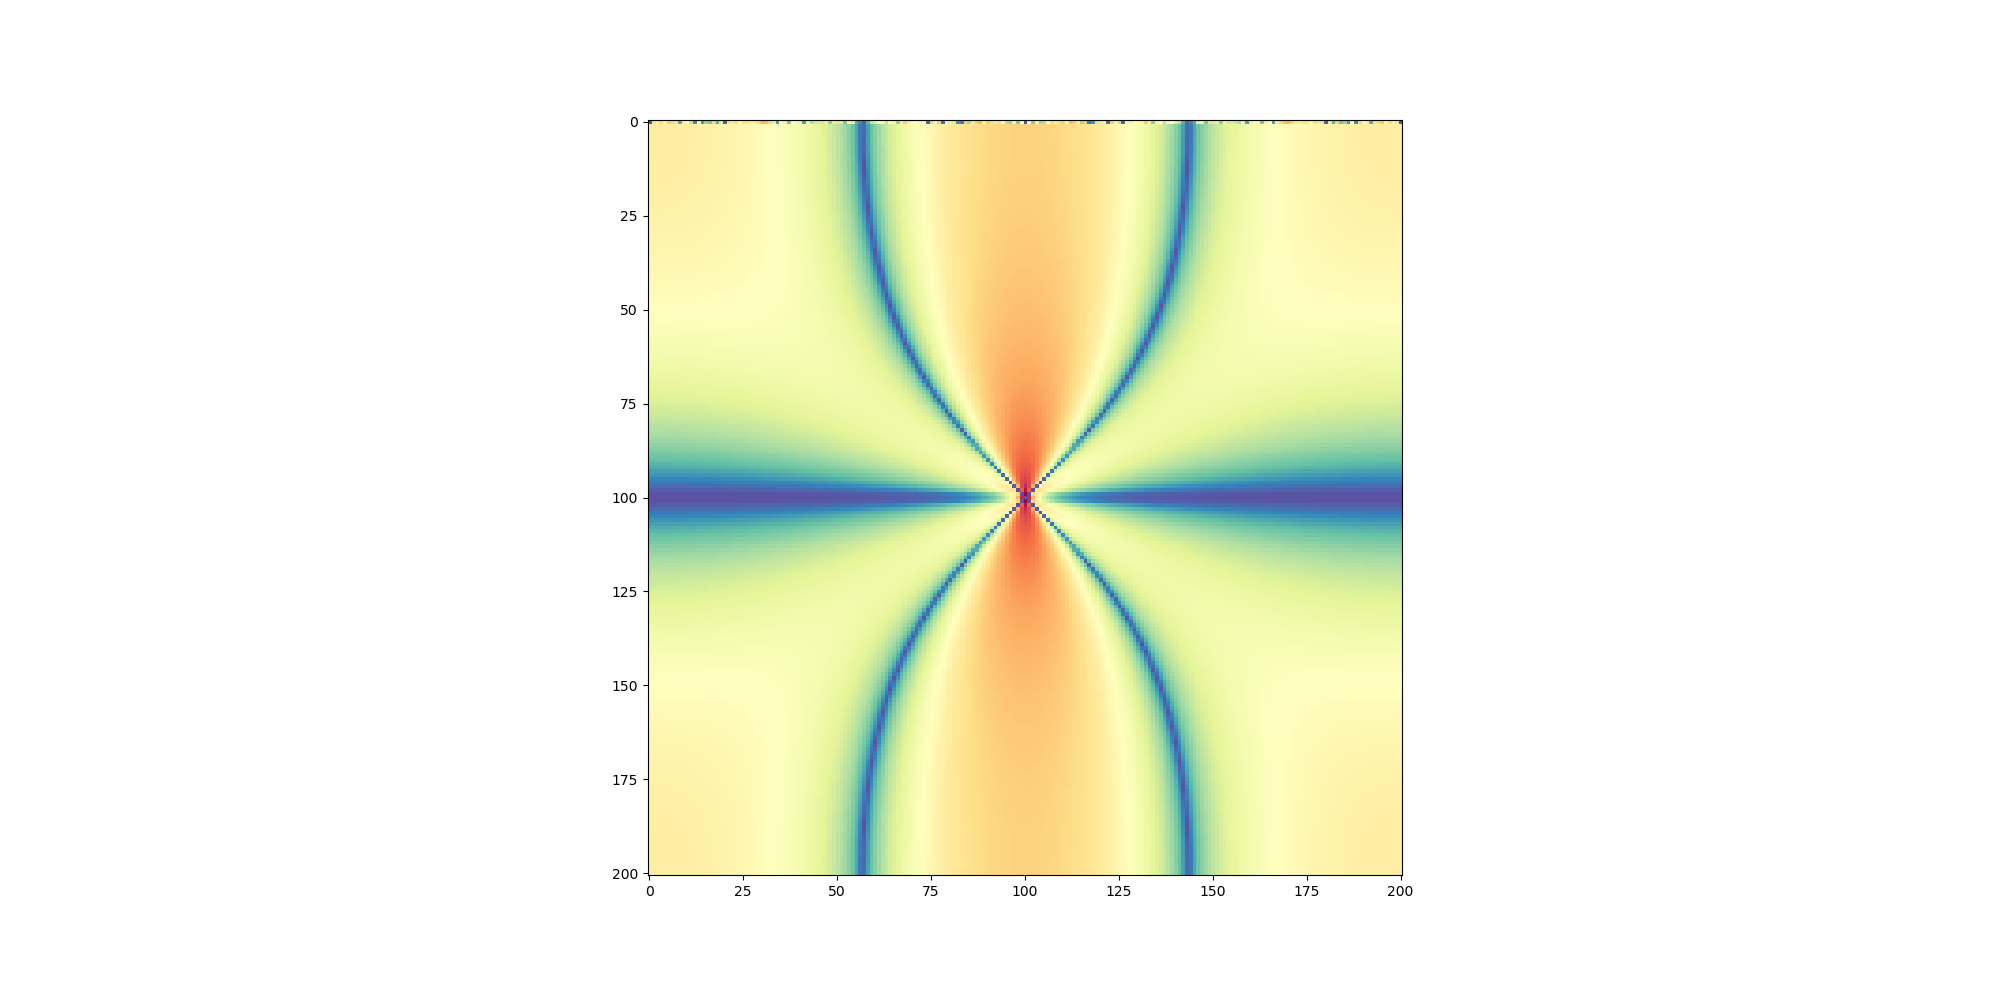
\includegraphics[width=1.\textwidth]{../week02/stess_field_orig.png}
\end{figure}

\par And zoomed in:

\begin{figure}[H]
\centering
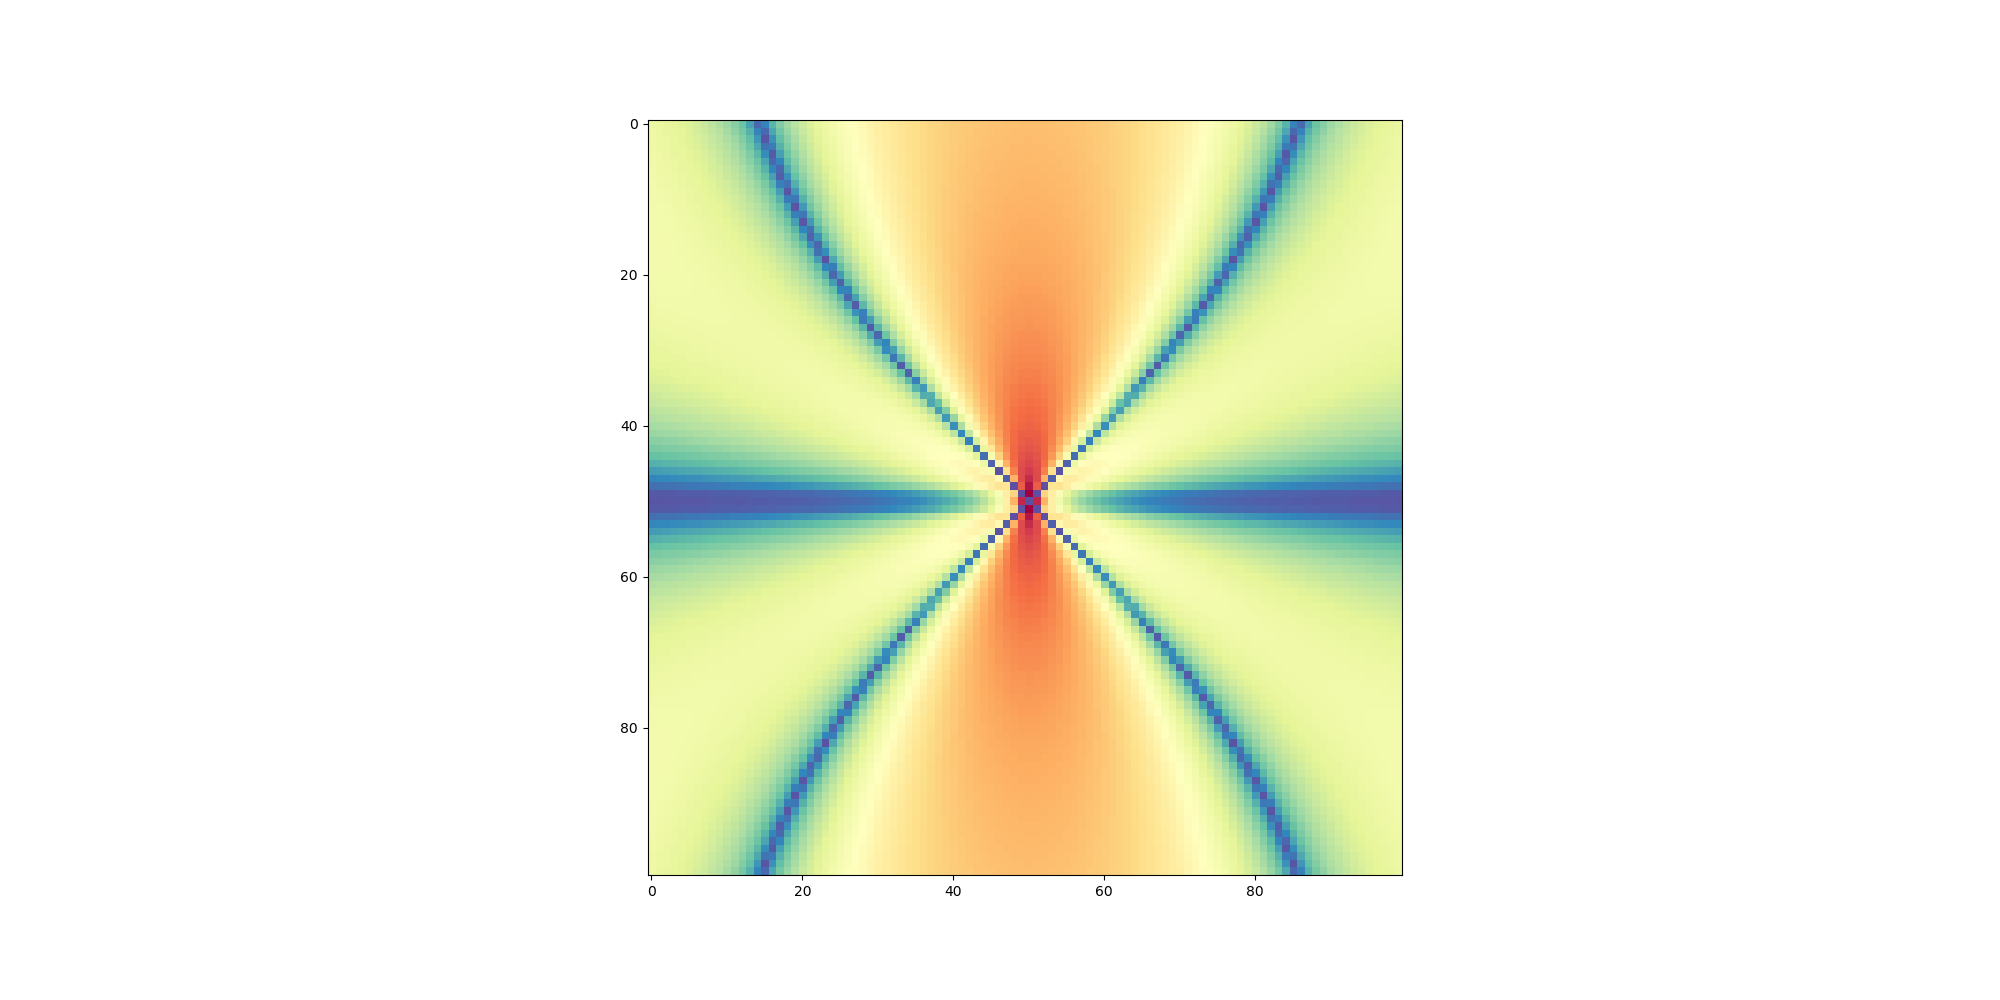
\includegraphics[width=1.\textwidth]{../week02/stess_field.png}
\end{figure}

\end{document}